\documentclass[A4paper, 11pt]{article}

\usepackage[UTF8]{ctex}
\usepackage{amsfonts}
\usepackage{amsmath} 
\usepackage{amssymb}
\usepackage{array}
\usepackage{booktabs}
\usepackage{bm}
\usepackage{cite}
\usepackage{colortbl}
\usepackage{enumerate}
\usepackage{extarrows}
\usepackage{float}
\usepackage{geometry}
\usepackage{graphics}
\usepackage{graphicx}
\usepackage{ifthen}
\usepackage{listings}
\usepackage{longtable}
\usepackage{multicol}
\usepackage{pgf}
\usepackage{pgfplots}
\usepackage{pifont}
\usepackage{pstricks}
\usepackage{pst-node}
\usepackage{pst-tree}
\usepackage{pythonhighlight}
\usepackage{setspace}
\usepackage{tabularx}
\usepackage{tikz}
\usepackage{tocloft}
\usepackage{wrapfig}

\geometry{left=2cm, right=2cm, top=2cm, bottom=2cm}

\definecolor{emph}{RGB}{0,100,141}

\newcommand{\tabincell}[2]{\begin{tabular}{@{}#1@{}}#2\end{tabular}}
\newcommand*{\circled}[1]{\lower.7ex\hbox{\tikz\draw (0pt, 0pt) circle (.5em) node {\makebox[1em][c]{\small #1}};}}
\newcommand{\sfrac}[2]{\mbox{\small$\dfrac{#1}{#2}$}}
\renewcommand{\geq}{\geqslant}
\renewcommand{\leq}{\leqslant}
\renewcommand{\vec}{\overrightarrow}
\renewcommand{\d}{\,\mathrm{d}}
\newcommand{\lto}{\longrightarrow}
\newcommand{\ex}{\exists\,}
\newcommand{\R}{\mathbb{R}}
\newcommand{\<}{\,\langle\,}
\renewcommand{\>}{\,\rangle}
\newcommand{\normuv}[1]{\big|{#1}(u,v)\big|^2}
\newcommand{\infint}{\int_{-\infty}^{+\infty}}
\newcommand{\hollowstar}{\text{\ding{73}}}
\newcommand{\fullstar}{\text{\ding{72}}}

\newcommand{\Pro}[1]{\textbf{\large{Problem #1}} \vspace*{1ex}}
\newcommand{\Sol}{\textbf{\textit{Sol.}}}
\newcommand{\Ckp}{\textbf{\textit{Checkpoints}}}
\newcommand{\Pt}[1]{\textcolor{emph}{(#1 \ifthenelse{\equal{#1}{1}}{point}{points})}}

% Scalars
\renewcommand{\a}{\alpha}
% Matrices
\newcommand{\A}{\bm{A}}
\newcommand{\B}{\bm{B}}
\newcommand{\C}{\bm{C}}
\newcommand{\E}{\bm{E}}
% Vectors
\renewcommand{\b}{\bm{b}}
\newcommand{\x}{\bm{x}}
\newcommand{\y}{\bm{y}}
\newcommand{\z}{\bm{z}}
\renewcommand{\u}{\bm{u}}
\renewcommand{\v}{\bm{v}}
\newcommand{\w}{\bm{w}}
\newcommand{\0}{\mathbf{0}}
\newcommand{\1}{\mathbf{1}}
% Spaces
\newcommand{\V}{\mathcal{V}}
\newcommand{\X}{\mathcal{X}}
\newcommand{\Y}{\mathcal{Y}}
\newcommand{\F}{\mathcal{F}}
\newcommand{\N}{\mathcal{N}}
\renewcommand{\S}{\mathcal{S}}
% Names
\renewcommand{\sp}{\text{span}}
\newcommand{\rank}{\text{rank}}
\newcommand{\range}{\mathcal{R}}
\newcommand{\tr}{\text{tr}}

\newcommand{\typeset}{
	\setlength{\parindent}{0pt}
	\setlength{\parskip}{1ex}
	\setlength{\abovedisplayskip}{1ex}
	\setlength{\belowdisplayskip}{1ex}
}

\newcommand{\headbox}{
	\renewcommand{\arraystretch}{1.33}
	\begin{tabular}{|l|l|}
		\hline
		Name       & \hspace*{9em} \\
		\hline
		Student ID & \hspace*{9em} \\
		\hline
	\end{tabular} \hspace{131pt}
	\begin{tabular}{r}
		\textsc{CS\,270:\;Digital\;Image\;Processing} \\
		\textbf{\Large{Quiz 1}} \\
	\end{tabular}
	
	\vspace*{6ex}
	\renewcommand{\arraystretch}{1}
}

\begin{document}
	
	\begin{spacing}{1.3}
		
		\typeset
		
		\textsc{\large{School\;of\;Information\;Science\;and\;Technology\\[2pt] ShanghaiTech\;University}}
		
		\vspace*{5ex}
		
		\textsc{\large{CS\,270:\;Digital\;Image\;Processing (Spring\;2024)}}
		
		\vspace*{2.5ex} \textbf{\huge{Assignment 1}}
		
		\vspace*{1.5ex} \textbf{\large{Due: 23:59, April 7, 2024}}
		
		\vspace*{1.5ex} \textbf{\large{Name: Yan Ruyue, No: 2020531005}}
		
		\vspace*{5ex}

		
		\Pro{1: Histogram Equalization}
		
		
		\begin{enumerate}[\bfseries(a)] \setlength{\parskip}{0.5ex} \vspace*{-2ex}
			\item Compute the histogram of \texttt{grain.tif} and show the histogram image in your report. (Built-in functions \texttt{hist} and \texttt{histogram} are not allowed). \Pt{5}
			\begin{center}
				
\includegraphics[width=10cm]{images/p1a.jpg}
			\end{center}
			
			\item Implement histogram equalization on \texttt{grain.tif}. Show the histogram equalized image and the histogram of equalized image in your report. (Built-in function \texttt{histeq} is not allowed). \Pt{10}
			
			\begin{center}
				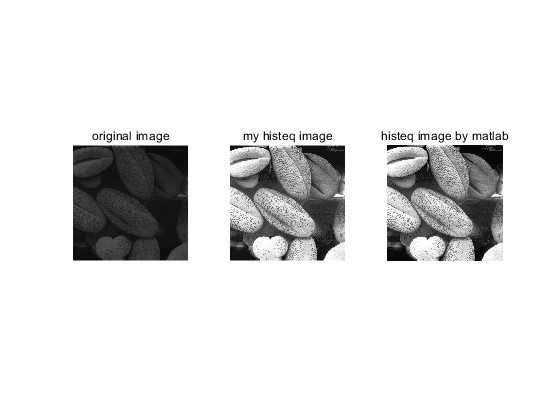
\includegraphics[width=10cm]{images/p1b_img.jpg}
			\end{center}
			\begin{center}
				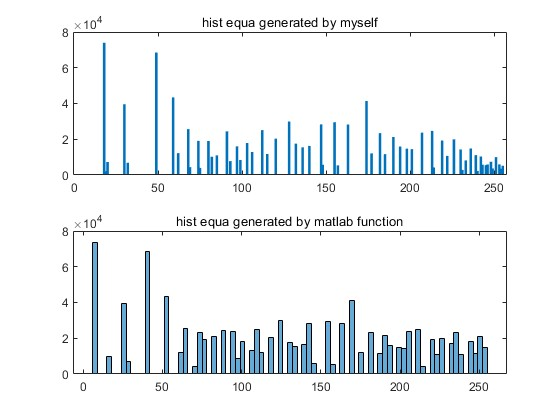
\includegraphics[width=10cm]{images/p1b_hist.jpg}
			\end{center}
			
			\item Implement contrast limited adaptive histogram equalization (CLAHE) on \texttt{tire.tif}, where you traverse every pixel with a $41 \times 41$ patch and process histogram equalization within each patch and update the center patch of $3 \times 3$. Each time you move the patch with a step of 1 pixel. The clip limit for CLAHE is 0.02, which means that after the normalization of the histogram, amplification above 0.02 should be clipped and evenly distributed to other parts of the histogram. Show the CLAHE processed images and corresponding histogram in your report. (Built-in function  \texttt{adapthisteq} is not allowed)  \Pt{20}
			
			\begin{center}
				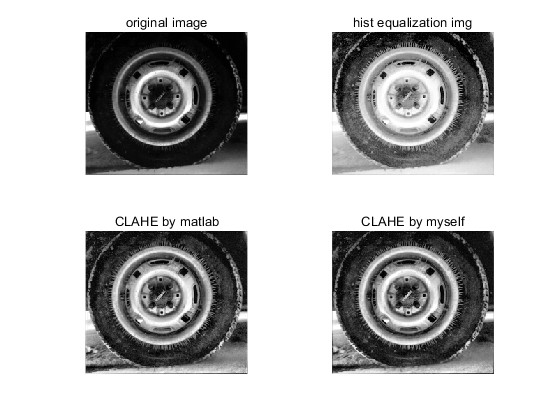
\includegraphics[width=10cm]{images/p1c_img.jpg}
			\end{center}
			\begin{center}
				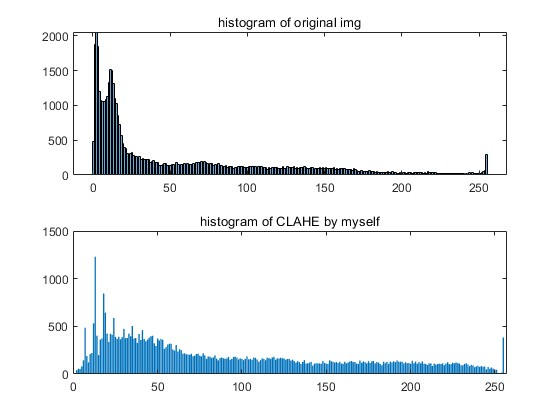
\includegraphics[width=10cm]{images/p1c_hist.jpg}
			\end{center}
		\end{enumerate}
	
		
		
		\newpage
		
		\Pro{2: Image Sharpening}
		
		(a) Apply the $3\times 3$ Laplacian kernels ($x$-direction and $y$-direction) on \texttt{moon.jpg} to obtain the details of the image. Since the Laplacian kernels are separable, please separate them into combinations of 1-D kernels and then apply them to the image sequentially. Show the separated Laplacian kernels and the corresponding processed images. (Implement your own \textbf{convolution} operator.) \Pt{15}
		\newline \\
		Applying Laplacian kernel, \\
		on x direction: $
			\begin{bmatrix}
				1 &-2 &1
			\end{bmatrix}$
		
		on y direction: $
		\begin{bmatrix}
			1 \\-2 \\1
		\end{bmatrix}$
		\begin{center}
			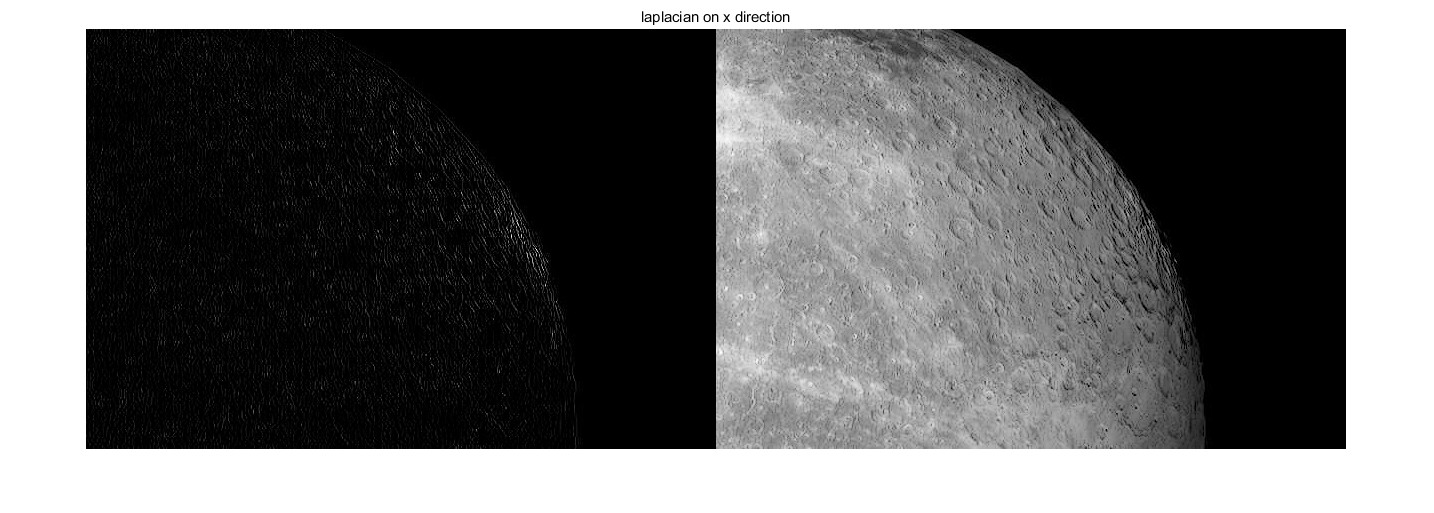
\includegraphics[width=15cm]{images/p2a_x.jpg}
		\end{center}
		\begin{center}
			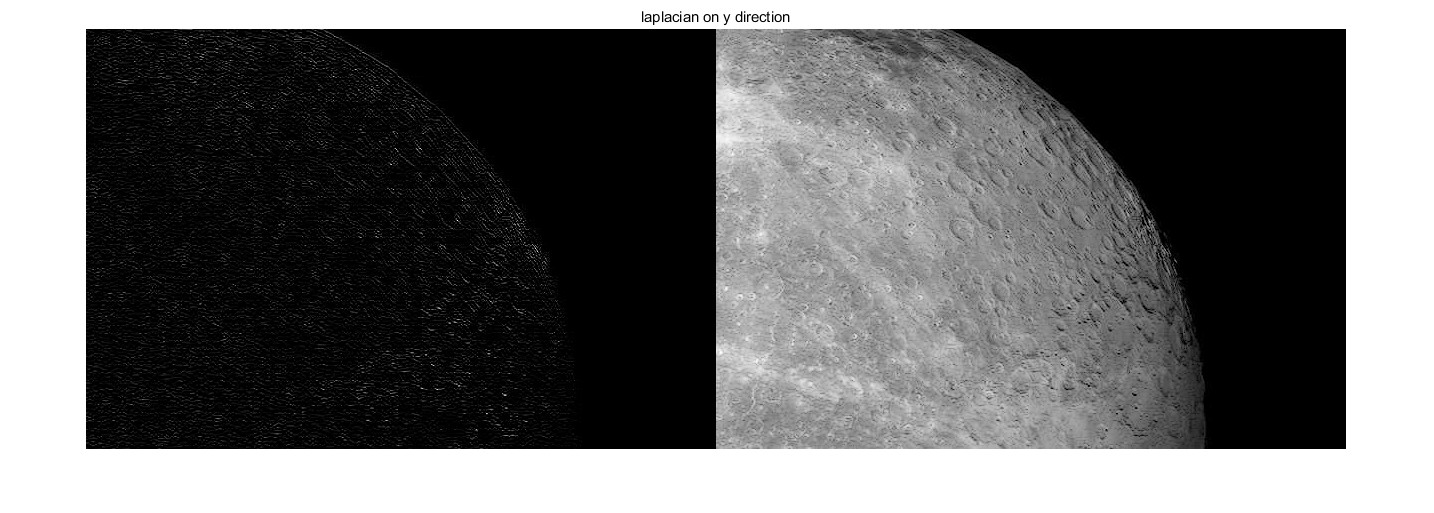
\includegraphics[width=15cm]{images/p2a_y.jpg}
		\end{center}
		\begin{center}
			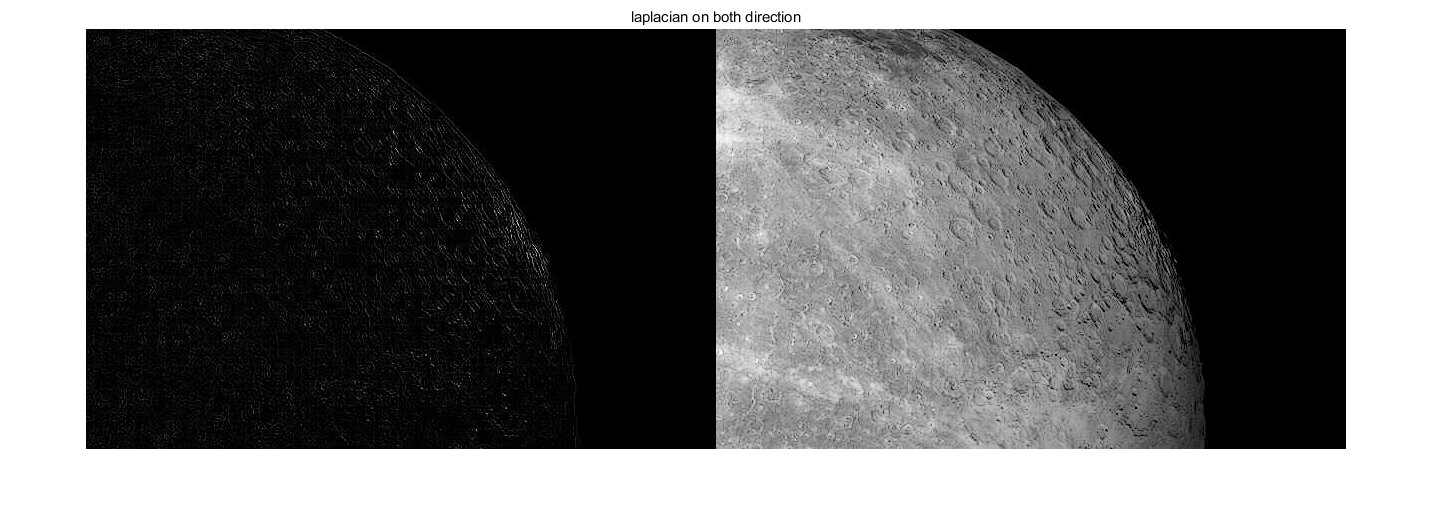
\includegraphics[width=15cm]{images/p2a.jpg}
		\end{center}
		
		(b) Apply the $3\times 3$ Laplacian kernels (not separated) to sharpen the image by 2-D convolution. Show the results in your report. \Pt{10}
		\newline \\
		Applying Laplacian kernel not seperated, $
		\begin{bmatrix}
			0 &1 &0\\
			1 &-4 &1\\
			0 &1 &0
		\end{bmatrix}$\\
		\begin{center}
			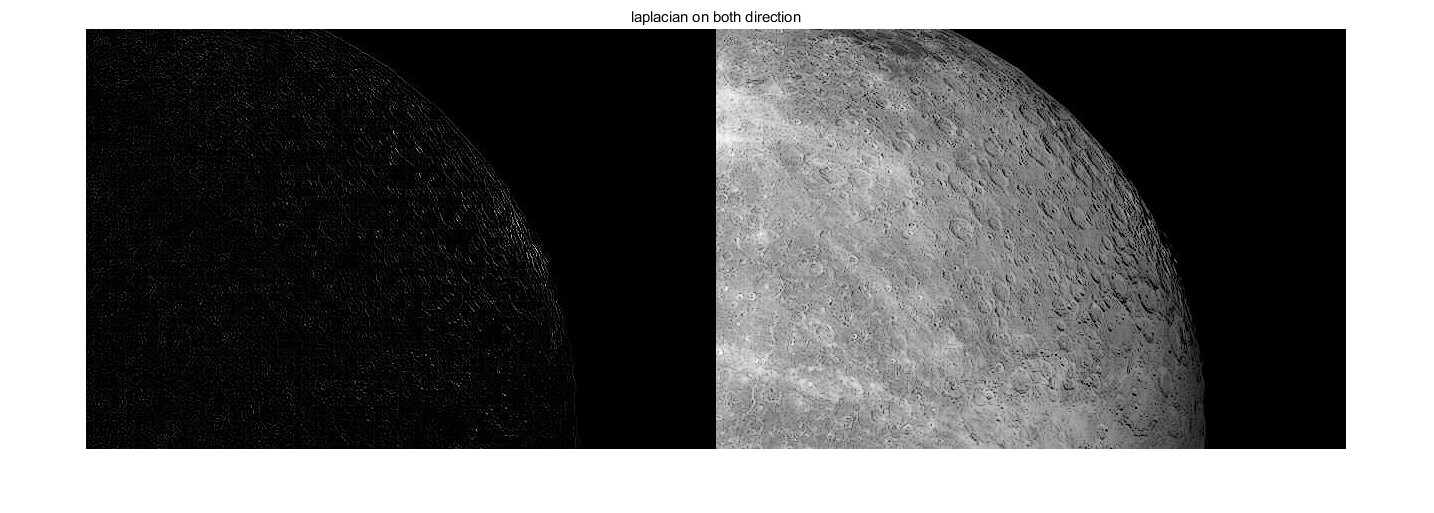
\includegraphics[width=15cm]{images/p2b.jpg}
		\end{center}
		
		(c) Use unsharpen mask to sharpen the image. Show the results in your report. \Pt{10}
		
		\hspace*{\fill} \\
		using unsharpen mask, \\
		$g_{mask}(x, y) = f(x, y) - \bar{f(x, y)}$, \\
		$g(x, y) = f(x, y) + k*g_{mask}(x, y), k = 1$
		\begin{center}
			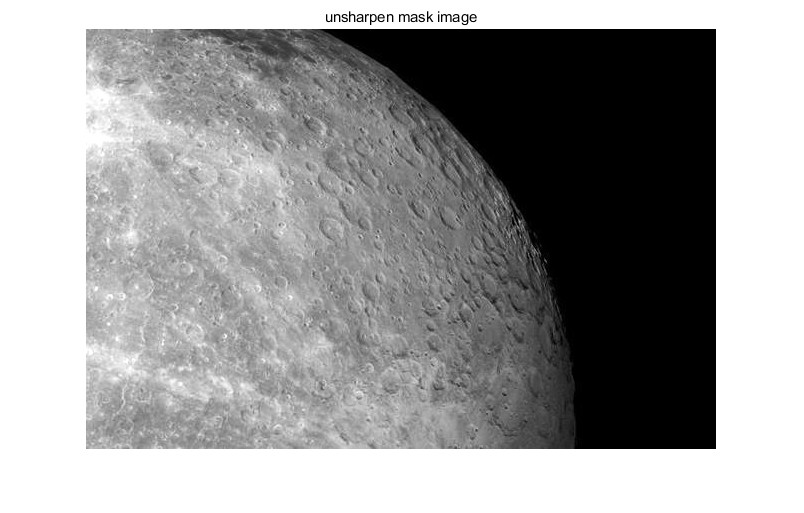
\includegraphics[width=15cm]{images/p2c.jpg}
		\end{center}
		
		
		
		\newpage
		
		
		\Pro{3: Nonlinear Filter}
		
		Apply the median filter and Gaussian filter to the image \texttt{lena\_noisy.tif}. In your report, Please show the images processed by the median filter and Gaussian filter respectively, and analyze the cause of the results. (Filtering operations cannot be implemented by calling functions, Hint: Choose the best kernel size you think, $\sigma = 1$) \Pt{30}
		
		\hspace*{\fill} \\
		median filter can filter salt-and-pepper noise better than gaussian filter\\
		the larger the kernel size is , the less noise, but the more blurry the image is
		
		\begin{center}
			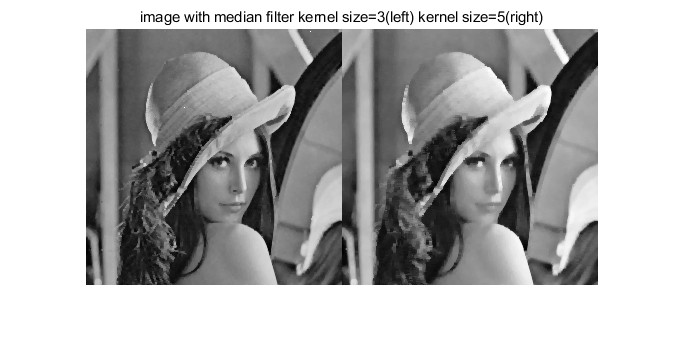
\includegraphics[width=15cm]{images/p3_median_filter.jpg}
		\end{center}
		\begin{center}
			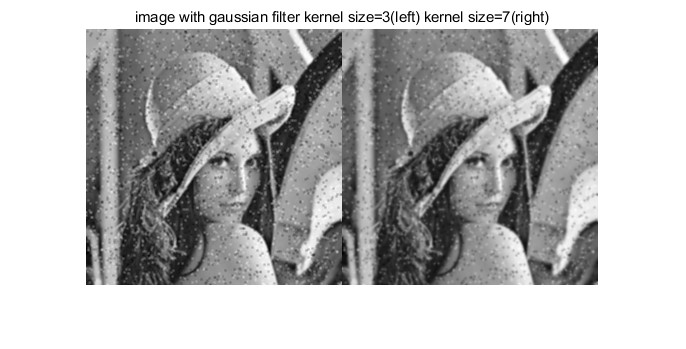
\includegraphics[width=15cm]{images/p3_gaussian_filter.jpg}
		\end{center}
		
		

		
		\newpage
		
		
		
		
	\end{spacing}
	
\end{document}